
\documentclass[11pt]{scrreprt}

\usepackage{graphicx} 
\usepackage{ucs}
\usepackage[utf8x]{inputenc}
\usepackage[T1]{fontenc}
\usepackage[ngerman]{babel}
\usepackage{amsmath}
\usepackage{fancyhdr}
 
\title{Matrix-Vektor-Produkt}
\author{Jonas Gütter\\ Matrikelnr 152127}
\pagestyle{fancy}

\begin{document}

\rhead[Parallel Computing 2]{Parallel Computing 2} 
\lhead[Jonas Gütter]{Jonas Gütter} 

\maketitle Im Rahmen der Aufgabe wurden verschiedene Implementierungen eines Matrix-Vektor-Produkts $A*x$ im Hinblick auf ihre Laufzeit miteinander verglichen. Folgende Implementierungsmöglichkeiten wurden betrachtet:

\begin{itemize}
\item Serielles Berechnen von $Ax$ auf der CPU
\item Serielles Berechnen von $A^T  x$ auf der CPU
\item Paralleles Berechnen von $Ax$ auf der GPU
\item Paralleles Berechnen von $A^T  x$ auf der GPU
\item Paralleles Berechnen von $Ax$ auf der GPU unter Nutzung von shared memory
\item Paralleles Berechnen von $A^T x$ auf der GPU unter Nutzung von shared memory
\item Paralleles Berechnen von $Ax$ auf der GPU unter Nutzung von shared memory und dynamischer Parallelisierung
\item Paralleles Berechnen von $A^T  x$ auf der GPU unter Nutzung von shared memory und dynamischer Parallelisierung
\end{itemize}
Abbildung \ref{im:times} zeigt die Laufzeiten der verschiedenen Implementierungen in Millisekunden für verschiedene Matrix-Größen. Bei der seriellen Implementierung zeigt sich, dass die Bildung des Produkts $Ax$ um etwa eine Größenordnung schneller ist, als die Bildung des Produkts $A^Tx$. Dies war auch zu erwarten, da bei einem Speicherzugriff mehrere aufeinanderfolgende Elemente in den Cache geladen werden, die bei $Ax$ auch direkt benötigt werden. Bei $A^Tx$ dagegen werden keine aufeinanderfolgenden Elemente benötigt, in jeder Iteration muss also ein neuer Zugriff auf den Hauptspeicher erfolgen. Bei der parallelen Berechnung ohne shared memory und dynamischer Parallelisierung verhält es sich genau andersherum, dort ist die Berechnung von $A^Tx$ deutlich schneller als die Berechnung von $Ax$. Dies liegt daran, dass jeder Thread eine Zeile der Matrix bearbeitet. Es werden also etwa gleichzeitig die ersten Elemente aller Zeilen abgerufen. Bei $A^Tx$ befindet sich ein großer Teil davon nach dem ersten Speicherzugriff bereits im Cache, daher wird in diesem Fall weniger Zeit benötigt. Die Implementierung mit Hilfe von shared memory weist im Vergleich dazu nur kleine Unterschiede zwischen $Ax$ und $A^Tx$ auf, die Variante $Ax$ ist jedoch durchgehend schneller. Da hier wieder mehrere Threads dieselbe Zeile bearbeiten, ist es wieder von Vorteil, dass aufeinanderfolgende Elemente sich unter Umständen bereits vor dem Speicherzugriff im Cache befinden. Dasselbe gilt für die Implementierung mit shared memory und dynamischer Parallelisierung.
\\
In den Abbildungen \ref{im:graph_full}, \ref{im:graph_smallx} und \ref{im:graph_smalltime} sind die verschiedenen Laufzeiten in Abhängigkeit von der Matrixgröße dargestellt. Vor allem in Abbildung \ref{im:graph_smalltime} ist zu erkennen, dass die parallele Berechnung ohne shared memory und ohne dynamischer Parallelisierung am wenigsten Zeit braucht. Dies liegt möglicherweise daran, dass für den Einsatz des shared memory das Programm teilweise wieder durch eine for-Schleife serialisiert wurde. Auch wurden atomare Operation eingesetzt, die die Laufzeit weiter erhöhen. Mit Abstand am langsamsten ist die serielle Implementierung in der Variante $A^Tx$, für Matrixgrößen ab 4096x4096 Einträgen wird auch der Einsatz der dynamischen Parallelisierung sehr langsam. Die Threadanzahl ist bei dieser Variante im Vergleich zu den anderen Implementierungen am größten, möglicherweise ist die Threadanzahl so groß, dass eine quasi-parallele Beabreitung durch Hyperthreading nicht mehr möglich ist.
\\
Die einfache parallele Berechnung des Produkts $A^Tx$ ohne weitere Konzepte ist also von den betrachteten Implementierungen am effektivsten. Der Einsatz des shared memmorys und der dynamischen Parallelisierung kann aber möglicherweise noch optimiert werden, so dass dort noch bessere Laufzeiten entstehen könnten.


\begin{figure}
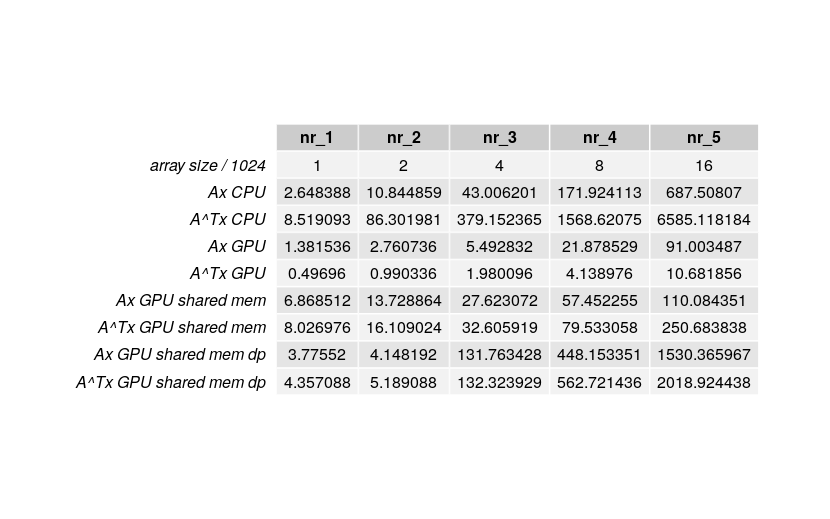
\includegraphics[width = \textwidth]{bilder/times.png}
\caption{Laufzeiten(ms) der verschiedenen Implementierungen für verschiedene Matrixgrößen}\label{im:times}
\end{figure}
\begin{figure}
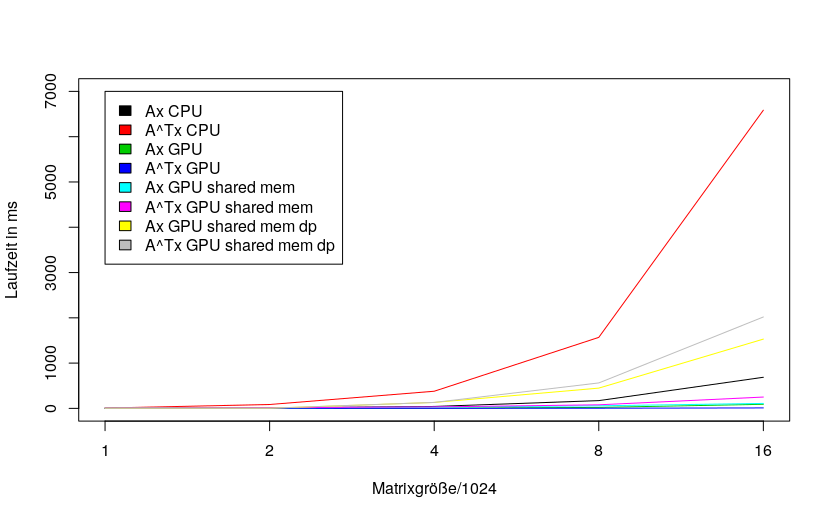
\includegraphics[width = \textwidth]{bilder/graph_full.png}
\caption{Entwicklung der Laufzeiten}
\label{im:graph_full}
\end{figure}
\begin{figure}
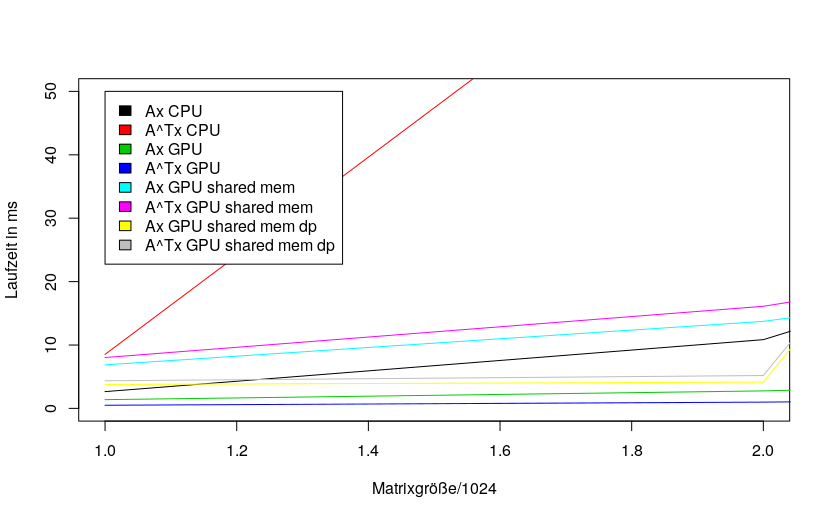
\includegraphics[width = \textwidth]{bilder/graph_smallx.png}
\caption{Entwicklung der Laufzeiten bei kleinen Problemgrößen}
\label{im:graph_smallx}
\end{figure}
\begin{figure}
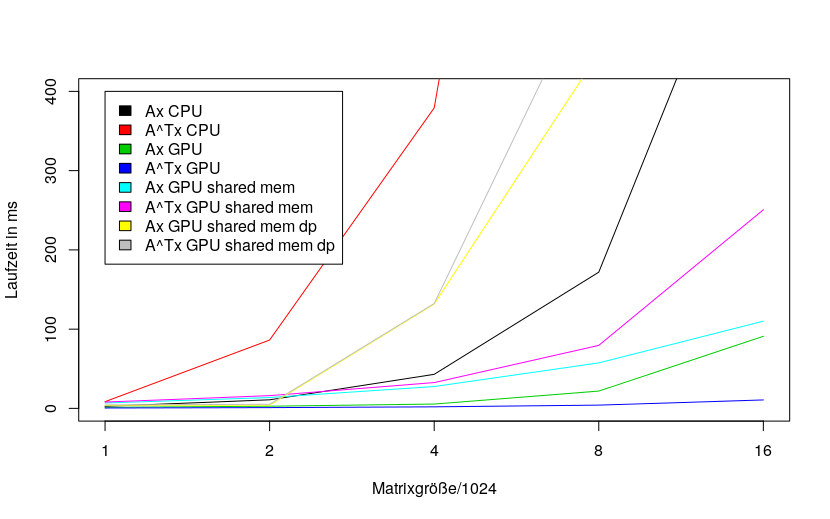
\includegraphics[width = \textwidth]{bilder/graph_smalltime.png}
\caption{Entwicklung der Laufzeiten unter 400 ms}
\label{im:graph_smalltime}
\end{figure}

\end{document}